\documentclass[14pt,a4paper]{report}  %紙張設定
\usepackage{xeCJK}%中文字體模組
%\setCJKmainfont{標楷體} %設定中文字體
\setCJKmainfont{MoeStandardKai.ttf}
%\newfontfamily\sectionef{Times New Roman}%設定英文字體
\newfontfamily\sectionef{Nimbus Roman}
\usepackage{enumerate}
\usepackage{amsmath,amssymb}%數學公式、符號
\usepackage{amsfonts} %數學簍空的英文字
\usepackage{graphicx, subfigure}%圖形
\usepackage{fontawesome5} %引用icon
\usepackage{type1cm} %調整字體絕對大小
\usepackage{textpos} %設定文字絕對位置
\usepackage[top=2.5truecm,bottom=2.5truecm,
left=3truecm,right=2.5truecm]{geometry}
\usepackage{titlesec} %目錄標題設定模組
\usepackage{titletoc} %目錄內容設定模組
\usepackage{textcomp} %表格設定模組
\usepackage{multirow} %合併行
%\usepackage{multicol} %合併欄
\usepackage{CJK} %中文模組
\usepackage{CJKnumb} %中文數字模組
\usepackage{wallpaper} %浮水印
\usepackage{listings} %引用程式碼
\usepackage{hyperref} %引用url連結
\usepackage{setspace}
\usepackage{lscape}%設定橫式
\lstset{language=Python, %設定語言
		basicstyle=\fontsize{10pt}{2pt}\selectfont, %設定程式內文字體大小
		frame=lines,	%設定程式框架為線
}
%\usepackage{subcaption}%副圖標
\graphicspath{{./../images/}} %圖片預設讀取路徑
\usepackage{indentfirst} %設定開頭縮排模組
\renewcommand{\figurename}{\Large 圖.} %更改圖片標題名稱
\renewcommand{\tablename}{\Large 表.}
\renewcommand{\lstlistingname}{\Large 程式.} %設定程式標示名稱
\hoffset=-5mm %調整左右邊界
\voffset=-8mm %調整上下邊界
\setlength{\parindent}{3em}%設定首行行距縮排
\usepackage{appendix} %附錄
\usepackage{diagbox}%引用表格
\usepackage{multirow}%表格置中
%\usepackage{number line}
%=------------------更改標題內容----------------------=%
\titleformat{\chapter}[hang]{\center\sectionef\fontsize{20pt}{1pt}\bfseries}{\LARGE 第\CJKnumber{\thechapter}章}{1em}{}[]
\titleformat{\section}[hang]{\sectionef\fontsize{18pt}{2.5pt}\bfseries}{{\thesection}}{0.5em}{}[]
\titleformat{\subsection}[hang]{\sectionef\fontsize{18pt}{2.5pt}\bfseries}{{\thesubsection}}{1em}{}[]
%=------------------更改目錄內容-----------------------=%
\titlecontents{chapter}[11mm]{}{\sectionef\fontsize{18pt}{2.5pt}\bfseries\makebox[3.5em][l]
{第\CJKnumber{\thecontentslabel}章}}{}{\titlerule*[0.7pc]{.}\contentspage}
\titlecontents{section}[18mm]{}{\sectionef\LARGE\makebox[1.5em][l]
{\thecontentslabel}}{}{\titlerule*[0.7pc]{.}\contentspage}
\titlecontents{subsection}[4em]{}{\sectionef\Large\makebox[2.5em][l]{{\thecontentslabel}}}{}{\titlerule*[0.7pc]{.}\contentspage}
%=----------------------章節的間距----------------------=%
\titlespacing*{\chapter} {0pt}{0pt}{18pt}
\titlespacing*{\section} {0pt}{12pt}{6pt}
\titlespacing*{\subsection} {0pt}{6pt}{6pt}
%=----------------------標題-------------------------=%             
\begin{document} %文件
\sectionef %設定英文字體啟用
\vspace{12em}
\begin{titlepage}%開頭
\begin{center}   %標題  
\makebox[1.5\width][s] %[s] 代表 Stretch the interword space in text across the entire width
{\fontsize{24pt}{2.5pt}國立虎尾科技大學}\\[18pt]
\makebox[1.5\width][s]
{\fontsize{24pt}{2.5pt}機械設計工程系}\\[18pt]
\sectionef\fontsize{24pt}{1em}\selectfont\textbf
{
\vspace{0.5em}
cd2023 2b-pj2bg12分組報告}\\[18pt]
%設定文字盒子 [方框寬度的1.5倍寬][對其方式為文字平均分分布於方框中]\\距離下方18pt
\vspace{1em} %下移
\fontsize{30pt}{1pt}\selectfont\textbf{網際足球場景設計}\\
\vspace{1em}
\sectionef\fontsize{30pt}{1em}\selectfont\textbf
{
\vspace{0.5em}
Web-based Football Scene Design}
 \vspace{2em}
%=---------------------參與人員-----------------------=%             
\end{center}
\begin{flushleft}
\begin{LARGE}

\hspace{32mm}\makebox[5cm][s]
{指導教授:\quad 嚴\quad 家\quad 銘\quad 老\quad 師}\\[6pt]
\hspace{32mm}\makebox[5cm][s]
{班\qquad 級:\quad 四\quad 設\quad 二\quad 乙}\\[6pt]
\hspace{32mm}\makebox[5cm][s]
{學\qquad 生:\quad 陳\quad 冠\quad 佑\quad(41023219)}
\\[6pt]
\hspace{32mm}\makebox[5cm][s]
{\hspace{36.5mm}陳\quad 冠\quad 翰\quad(41023221)}\\[6pt]
\hspace{32mm}\makebox[5cm][s]
{\hspace{36.5mm}陳\quad 奕\quad 倫\quad(41023222)}\\[6pt]
\hspace{32mm}\makebox[5cm][s]
{\hspace{36.5mm}陳\quad 瑨\quad 維\quad(41023228)}\\[6pt]
\hspace{32mm}\makebox[5cm][s]

%設定文字盒子[寬度為5cm][對其方式為文字平均分分布於方框中]空白距離{36.5mm}\空白1em
\end{LARGE}
\end{flushleft}
\vspace{6em}
\fontsize{18pt}{2pt}\selectfont\centerline{\makebox[\width][s]
{中華民國\hspace{3em} 
112 \quad 年\quad 5\quad 月}}
\end{titlepage}
\newpage

%=------------------------摘要-----------------------=%
\renewcommand{\baselinestretch}{1.5} %設定行距
\pagenumbering{roman} %設定頁數為羅馬數字
\clearpage  %設定頁數開始編譯
\sectionef
\addcontentsline{toc}{chapter}{摘~~~要} %將摘要加入目錄
\begin{center}
\LARGE\textbf{摘~~要}\\
\end{center}
\begin{flushleft}
\fontsize{14pt}{20pt}\sectionef\hspace{12pt}\quad 由於矩陣計算、自動求導技術、開源開發環境、多核GPU運算硬體等這四大發展趨勢,促使AI領域快速發展,藉由這樣的契機,將實體機電系統透過虛擬化訓練提高訓練效率,再將訓練完的模型應用到實體上。\\[12pt]

\fontsize{14pt}{20pt}\sectionef\hspace{12pt}\quad 此專題是運用實體冰球對打機,將其導入CoppeliaSim模擬環境並給予對應設置,將其機電系統簡化並運用Open AI Gym進行訓練,找到適合此系統的演算法後,再到CoppeliaSim模擬環境中進行測試演算法在實際運用上的可行性。並嘗試透過架設伺服器將CoppeliaSim影像串流到網頁供使用者觀看或操控。\\[12pt]

\end{flushleft}
\begin{center}
\fontsize{14pt}{20pt}\selectfont 關鍵字: 類神經網路、強化學習、\sectionef CoppeliaSim、OpenAI Gym
\end{center}
\newpage
%=--------------------Abstract----------------------=%
\renewcommand{\baselinestretch}{1.5} %設定行距
\addcontentsline{toc}{chapter}{Abstract} %將摘要加入目錄
\begin{center}
\LARGE\textbf\sectionef{Abstract}\\
\begin{flushleft}
\fontsize{14pt}{16pt}\sectionef\hspace{12pt}\quad Due to the four major development trends of multidimensional arrays  computing, automatic differentiation, open source development environment, and multi-core GPUs computing hardware. The rapid development of the AI field has been promoted. In view of this development, the physical mechatronic systems can gain machine learning efficiency through their simulated virtual system training process. And afterwards to apply the trained model into real mechatronic systems.\\[12pt]

\fontsize{14pt}{16pt}\sectionef\hspace{12pt}\quad This project is to use the physical air hockey to play machine, introduce it into the CoppeliaSim simulation environment and give the corresponding settings, simplify its electromechanical system and use Open AI Gym for training, find an algorithm suitable for this system, and then perform it in the CoppeliaSim simulation environment Feasibility of testing algorithm in practical application. And try to stream CoppeliaSim images to web pages for users to watch or manipulate by setting up a server.\\
\end{flushleft}
\begin{center}
\fontsize{14pt}{16pt}\selectfont\sectionef Keyword:  nerual network、reinforcement learning、 CoppeliaSim、OpenAI Gym
\end{center}
\newpage
\renewcommand{\baselinestretch}{1.5} %設定行距

%=------------------------誌謝----------------------=%
\begin{center}	
\addcontentsline{toc}{chapter}{誌~~~謝}
\LARGE\textbf{誌~~謝}\\
\end{center}
\begin{center}
\begin{flushleft}
\fontsize{14pt}{20pt}\sectionef\hspace{12pt}\quad 在此鄭重感謝製作以及協助本分組報告完成的所有人員,首先向嚴家銘老師致謝,他解決我們的各種提問,甚至從來沒有不耐煩,總是貼心為我們找出最佳解答。再來是第 12 組的 41023251 鄭立揚同學,他給了我們全方位的支援,提供我們解決問題的建議,最後是由本分組成員同心協力才得以完成本報告,特此感謝

\end{flushleft}
\newpage
%=------------------------目錄----------------------=%
\renewcommand{\contentsname}{\centerline{\fontsize{18pt}{\baselineskip}\selectfont\textbf{目\quad 錄}}}
\tableofcontents  %目錄產生
\newpage
------------內容----------------------=%

\chapter{更新網站步驟}
\section{詳細步驟說明}


 1.個人的fork倉儲點選sync fork\\

2.輸入git pull\\

3.進行編輯\\

4.acp\\

5.從個人fork 倉儲Open pull request\\

6.回到整組倉儲merge pull request\\


\chapter{W9}


\section{W9\_41023219}

心得:剛開始在下載完老師給的程式檔後,還是不知道怎麼動起來,好在最後有發現問題,讓機器人得以成功操控,非常有成就感。



\section{W9\_41023221}

心得:剛開始的時候遇到許多困難與錯誤,最後發現是缺失模組導致無法連線,所幸最後有成功解決,成功連線後成就感十足。



\section{W9\_41023222}

心得:感謝隊友在旁邊指導,用完真的很有成就感。

\section{W9\_41023228}

心得:一開始,不知道怎麼用,後來,上老師的網站查找怎麼做後,才知道要載入子模組,在控制台打上ipconfig找到主機的ip,輸入到.py檔中,連上組員電腦時,超興奮。


\chapter{W10}
\section{第一題}
What is zmqRemoteAPI, and how does it relate to CoppeliaSim?

答

1.zmqRemoteAPI是 ZeroMQ 的遠程 API 通訊協議,用於在不同的程序之間進行通訊和數據傳輸。

2.可使CoppeliaSim進行遠端連接操控。


\section{第二題}
How do you establish a connection between a Python script and CoppeliaSim using zmqRemoteAPI?

答

python先下載zmq子模組,利用port:23000連接


\section{第三題}
What are some common use cases for zmqRemoteAPI in CoppeliaSim?

答

在 CoppeliaSim 中,zmqRemoteAPI 可以用於以下一些常見的應用場景:

控制機器人:zmqRemoteAPI 可以用於控制機器人在 CoppeliaSim中的運動和行為,包括設置關節位置、速度和力矩等參數,控制機器人的運動軌跡和姿態,以及獲取機器人的感測器數據和影像信息等。

編寫自動化測試:zmqRemoteAPI 可以幫助使用者編寫自動化測試脚本,測試機器人和其他物體的運動和行為,並驗證機器人的控制算法和程序的正確性。

設計自主導航系統:zmqRemoteAPI 可以用於設計自主導航系統,通過控制機器人的運動和行為來實現自主導航,並在 CoppeliaSim 中進行仿真測試。

進行物體檢測和跟蹤:zmqRemoteAPI 可以用於設計物體檢測和跟蹤系統,通過獲取 CoppeliaSim 中的影像數據和感測器數據來實現物體檢測和跟蹤功能。

zmqRemoteAPI 可以幫助使用者更加靈活方便控制 CoppeliaSim 中的機器人和物體。


\section{第四題}
What are the advantages and disadvantages of using zmqRemoteAPI compared to other methods of communication between Python and CoppeliaSim?

答

優點:

快速和高效:zmqRemoteAPI使用ZeroMQ消息庫,以其快速和高效的消息傳遞能力而聞名。
易於使用:zmqRemoteAPI是一個簡單易用的API,提供了一系列函數,可從Python腳本中控制模擬。
跨語言支持:zmqRemoteAPI是一種跨語言協議,因此您可以使用任何支持ZeroMQ的編程語言。
支持多個連接:zmqRemoteAPI支持多個連接,因此您可以將多個客戶端連接到單個CoppeliaSim實例。
缺點:

功能受限:儘管zmqRemoteAPI提供了一系列函數來控制CoppeliaSim,但與其他通信方法(如ROS或Python的Coppeliasim庫)相比,其功能受限。
上手難度高:zmqRemoteAPI需要一些ZeroMQ和socket編程的知識,這對於新手用戶來說可能不太容易使用。
可能出現錯誤:如果通信未正確配置,zmqRemoteAPI容易出現錯誤,這可能會導致消息丟失或模擬停滯等問題。
彈性較小:與其他通信方法相比,zmqRemoteAPI的自定義彈性較小,因為它依賴於預定義的一組函數。

\section{第五題}
Can you give an example of a project or task that you could complete using zmqRemoteAPI in CoppeliaSim?

答

1.開啟CoppeliaSim

2.選取場景

3.尋找主機IP位置

4.更改城市中的連結為至於上步驟之主機位置

5.開始連結


\section{小組工作分配}
41023219: 

設計零件導入場景。

41023221: 

討論查詢程式。

41023222: 

場景建設。

41023228: 

討論與設計程式,製作亂數。
\section{2b網站順序亂數}
\begin{lstlisting}[language=Python, frame=single, numbers=left, captionpos=b, basicstyle=\ttfamily\small, showstringspaces=false, breaklines=true, tabsize=4, xleftmargin=15pt]
from browser import html, document
import random
bcd_tem = "https://mdecd2023.github.io/2b2-pj2bg"
bgithub = "https://github.com/mdecd2023/2b2-pj2bg"
brython_div = document["brython_div1"]
#  亂數範圍從1到16
grp = []
for i in range(1, 17):
    grp.append(i)
random.shuffle(grp)
for i in grp:
    url = bcd_tem + str(i)
    github = bgithub + str(i)
    brython_div <= html.A("pj2bg"+str(i), href=url)
    brython_div <= " ("
    brython_div <= html.A("repo", href=github)
    brython_div <= ")"
    brython_div <= html.BR()
\end{lstlisting}
\chapter{W11}


\section{41023234}
自評分數:65\\這次四人分組 我主要把  組別亂數生成  完成把  感測器、場景、記分板  生成並運轉出來


\section{41023247}
自評分數:62\\分在這次的分組作業,學到了如何解決合併時所產生的問題,同時,在本次的模擬中提供了場地,也更了解如何將cad圖檔轉檔進CoppeliaSim。而在這次的作業裡,我們發現到球門只會感應到機器人而不是球,一開始對於這個問題沒有任何想法解決,,直到詢問班上的別組同學,才知道要將機器人與球的物理性質更改,這才解決了這個煩人的問題。

\section{41023251}
自評分數:65\\負責完成latex分組報告。在4人協作的pj2開始時主要負責研究如何操作pull request,擬出一套操作步驟置於組內H1頁面。同時維護網站時期主要研究如何多人同時維護網站,常與54號同學於放學後留下研究。
因為W9內H2頁面標題與W11重複,導致讀取content資料夾內html檔案時會有兩個相同檔名。因此將W9內之H2頁面重新命名。

\section{41023254}
我在這次四人協同的課程中主要負責程式的工作,在大家pull requests發生衝突時也會解決衝突,解決衝突的方法來自和51號同學放學後一次又一次的同時上傳測試。\\	自評:60
%=---------------附錄-----------------=%
\addcontentsline{toc}{chapter}{附錄} %新增目錄名稱

\newpage
%=-------------作者簡介-----------------=%
    \addcontentsline{toc}{chapter}{作者簡介}
    \begin{center}
	\fontsize{20pt}{0em}\selectfont \bf{作者簡介}\\
	\end{center}	
	{\begin{textblock}{6}(0,0.5)
	\begin{figure}
	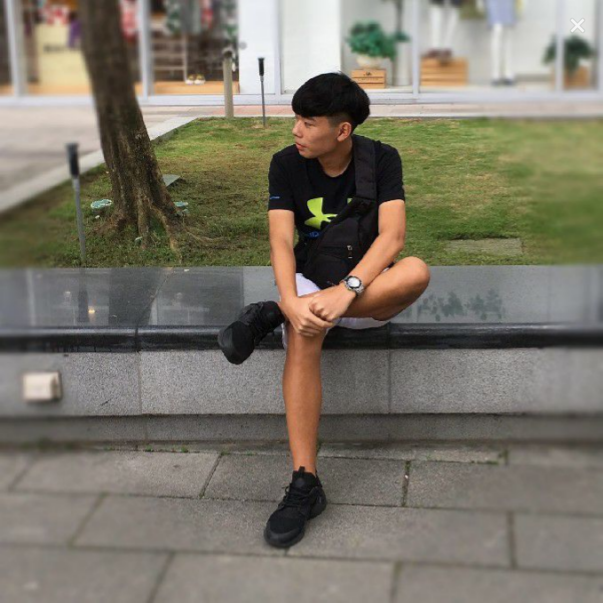
\includegraphics[width=1.25in]{41023219}  %作者照片
	\end{figure}
	\end{textblock}}
	{\renewcommand\baselinestretch{0.99}\selectfont %設定以下行距
	{\begin{textblock}{15}(3.5,0.7)%{寬度}(以左上角為原點之右移量,下移量)
	\noindent\fontsize{14pt}{0em}\selectfont \makebox[4em][s]{姓名}\enspace:\enspace
    \fontsize{14pt}{0em}\selectfont \makebox[4em][s]{陳冠佑}\\     \hspace*{\fill} \\
    \fontsize{14pt}{0em}\selectfont \makebox[4em][s]{學號}\enspace:\enspace
    \fontsize{14pt}{0em}\selectfont \makebox[4em][s]{41023219} \\ %\makebox為文本盒子
    \hspace*{\fill} \\
    \fontsize{14pt}{0em}\selectfont \makebox[4em][s]{就讀學校}\enspace:\enspace
    \fontsize{14pt}{0em}\selectfont \makebox[9em][s]{國立虎尾科技大學}\\
    \fontsize{14pt}{0em}\selectfont \makebox[5em][s]{\quad}\enspace\enspace
    \fontsize{14pt}{0em}\selectfont \makebox[8em][s]{機械設計工程系}\\
    \hspace*{\fill} \\
    \fontsize{14pt}{0em}\selectfont \makebox[4em][s]{經歷}\enspace:\enspace
    \end{textblock}}}
   % \hspace*{\fill} \\
   \vspace{2em}
	{\begin{textblock}{6}(0,2.3)
	\begin{figure}
	
\includegraphics[width=1.15in]{41023221}  %作者照片
    \end{figure}
    \end{textblock}}
    {\renewcommand\baselinestretch{0.99}
    \selectfont %設定以下行距
    {\begin{textblock}{15}(3.5,2.5) %{寬度}(以左上角為原點之右移量,下移量)
\noindent\fontsize{14pt}{0em}\selectfont \makebox[4em][s]{姓名}\enspace:\enspace
\fontsize{14pt}{0em}\selectfont \makebox[4em][s]{陳冠翰}\\ 
\hspace*{\fill} \\
\fontsize{14pt}{0em}\selectfont \makebox[4em][s]{學號}\enspace:\enspace
\noindent\fontsize{14pt}{0em}\selectfont \makebox[4em][s]{41023221} \\ 
\hspace*{\fill} \\
\fontsize{14pt}{0em}\selectfont \makebox[4em][s]{就讀學校}\enspace:\enspace
\fontsize{14pt}{0em}\selectfont \makebox[9em][s]{國立虎尾科技大學}\\
\fontsize{14pt}{0em}\selectfont \makebox[5em][s]{\quad}\enspace\enspace
\fontsize{14pt}{0em}\selectfont \makebox[8em][s]{機械設計工程系}\\
\hspace*{\fill} \\
\fontsize{14pt}{0em}\selectfont \makebox[4em][s]{經歷}\enspace:\enspace
    \end{textblock}}}
    %\hspace*{\fill} \\
    \vspace{2em}
    {\begin{textblock}{6}(0,4.1)
    \begin{figure}
        
\includegraphics[width=1.15in]{41023222} %{}內是圖片文件的相對路徑
    \end{figure}
    \end{textblock}}
    {\renewcommand\baselinestretch{0.99}\selectfont %設定以下行距
    {\begin{textblock}{15}(3.5,4.3) %{寬度}(以左上角為原點之右移量,下移量)
\noindent\fontsize{14pt}{0em}\selectfont \makebox[4em][s]{姓名}\enspace:\enspace%\noindent指定首行不進行縮排
\fontsize{14pt}{0em}\selectfont \makebox[4em][s]{陳奕倫}\\ 
\hspace*{\fill} \\
\noindent\fontsize{14pt}{0em}\selectfont \makebox[4em][s]{學號}\enspace:\enspace
\noindent\fontsize{14pt}{0em}\selectfont \makebox[4em][s]{41023222} \\ %\makebox為文本盒子
\hspace*{\fill} \\
\noindent\fontsize{14pt}{0em}\selectfont \makebox[4em][s]{就讀學校}\enspace:\enspace
\noindent\fontsize{14pt}{0em}\selectfont \makebox[9em][s]{國立虎尾科技大學}\\
\noindent\fontsize{14pt}{0em}\selectfont \makebox[5em][s]{\quad}\enspace\enspace
\noindent\fontsize{14pt}{0em}\selectfont \makebox[8em][s]{機械設計工程系}\\
\hspace*{\fill} \\
\noindent\fontsize{14pt}{0em}\selectfont \makebox[4em][s]{經歷}\enspace:\enspace
    \end{textblock}}}
   % \hspace*{\fill} \\
   \vspace{2em}
    {\begin{textblock}{6}(0,5.9)
    \begin{figure}
        
\includegraphics[width=1.15in]{41023228} %{}內是圖片文件的相對路徑
    \end{figure}
    \end{textblock}}
    {\renewcommand\baselinestretch{0.99}\selectfont %設定以下行距
    {\begin{textblock}{15}(3.5,6.1) %{寬度}(以左上角為原點之右移量,下移量)
\noindent\noindent\fontsize{14pt}{0em}\selectfont \makebox[4em][s]{姓名}\enspace:\enspace
\noindent\fontsize{14pt}{0em}\selectfont \makebox[4em][s]{陳瑨維}\\ \hspace*{\fill} \\
\noindent\fontsize{14pt}{0em}\selectfont \makebox[4em][s]{學號}\enspace:\enspace
\noindent\fontsize{14pt}{0em}\selectfont \makebox[4em][s]{41023228} \\ \hspace*{\fill} \\
\noindent\fontsize{14pt}{0em}\selectfont \makebox[4em][s]{就讀學校}\enspace:\enspace
\noindent\fontsize{14pt}{0em}\selectfont \makebox[9em][s]{國立虎尾科技大學}\\
\noindent\fontsize{14pt}{0em}\selectfont \makebox[5em][s]{\quad}\enspace\enspace
\noindent\fontsize{14pt}{0em}\selectfont \makebox[8em][s]{機械設計工程系}\\
\hspace*{\fill} \\
\noindent\fontsize{14pt}{0em}\selectfont \makebox[4em][s]{經歷}\enspace:\enspace
    \end{textblock}}}
    %\hspace*{\fill} \\

\newpage
%=----------------書背----------------------=%
\pagestyle{empty}%設定沒有頁眉和頁腳
\begin{center}
\fontsize{0.001pt}{1pt}\selectfont .\\
\vspace{4em}
\fontsize{30pt}{30pt}\selectfont 【13】 \\
\fontsize{20pt}{20pt}\selectfont
\vspace{0.5em}
分\\
類\\
編\\
號\\
\vspace{0.5em}
\hspace{-0.5em}:\\
\vspace{0.5em}
\rotatebox[origin=cc]{270}{\sectionef\LARGE \textbf{pj2bg12}}\\ %旋轉
\vspace{0.5em}
網\\
際\\
足\\
球\\
場\\
景\\
設\\
計\\
\vspace{2em}
一\\
一\\
二\\
級\\

\end{center}
%\newpage
%\begin{landscape}  %橫式環境
%\begin{center}
%\fontsize{0.001pt}{1pt}\selectfont .
%\vspace{70mm}
%\rotatebox[origin=cc]{90}{\LARGE 【14】}\rotatebox[origin=cc]%{180}{\LARGE 1-2-APP-8765} %旋轉
%\end{center}
%\end{landscape}
\end{document}
